\chapter{The memory}
\label{ch:PGMEMORY}
The PostgreSQL memory at first sight looks simple. If compared with the complex structures implemented in 
the other DBMS to a careless reader could seem rudimentary. However, the memory and in particular the 
shared buffers implementation is complex and sophisticated. This chapter will dig down deep into the 
PostgreSQL's memory.

\section{The shared buffer}
The shared buffer is a segment allocated at cluster's startup. Its size is determined by the GUC parameter 
shared\_buffers and the size can be changed only restarting the cluster. The shared buffer is used 
to manage the data pages as seen in \ref{sec:CLUBACKEND}, which are called buffers when loaded in 
rhw memory. Having a RAM segment is not uncommon in the database universe. Is a rapid exchange 
area where the buffers are kept across the sessions and keeps the data near the CPU. Like his competitors 
PostgreSQL strives to keep in memory what is important and not everything. In the era of the 
\textit{in memory databases} this could seems an obsolete concept. Unfortunately the truth is that the 
resources, and so the money, are not infinite. And after all an in memory database is a database without the D IN 
the ACID. Before digging into the technical details we'll have a look 
to the history of the memory manager. The way PostgreSQL sticks an elephant into a small car without 
Timelord technology.

Back in the old days PostgreSQL was quite rudimentary. The version 7.4 did not had tablespaces, it was 
without a mechanism to prevent the XID wraparound failure (except for the routine vacuuming of course) 
and the memory manager was a simple LRU buffer. Since then the algorithm evolved and became a very efficient system to 
cache effectively the buffers. We'll look briefly to the free space manager's history. 

\subsection{PostgreSQL 7.4, the LRU list}
In PostgreSQL 7.4 the free space in the shared buffer was managed using a simple last recently used list implemented using a FIFO list.

When a page is first request from disk the buffer manager puts it into the first buffer in the free LRU 
list. If the first buffer is used by another page the list is shifted by one unity and the eventual last 
page in the list is discarded. If a page in the list is requested again is put back into the first buffer 
and so on. This simple approach worked quite well with some unpleasant effects. After all the buffer is 
shared and is not uncommon to have more than one database on the same cluster, each database different 
design and purposes. This worked quite bad with the LRU list causing unnecessary disk IO because the 
buffers were evicted without considering their usage frequency. This lead us to the tale of the buffer.


\subsection{PostgreSQL 8.0, the 2q}
With the revolutionary PostgreSQL 8.0 the PostgreSQL global team introduced a different memory manager, the two 
queues.\newline 
The buffer manager keeps three list of pointers to the buffer pages called cache directory blocks (CDB) T1,T2 and 
B1. Each list is a simple FIFO buffer.\newline

\begin{figure}[H]
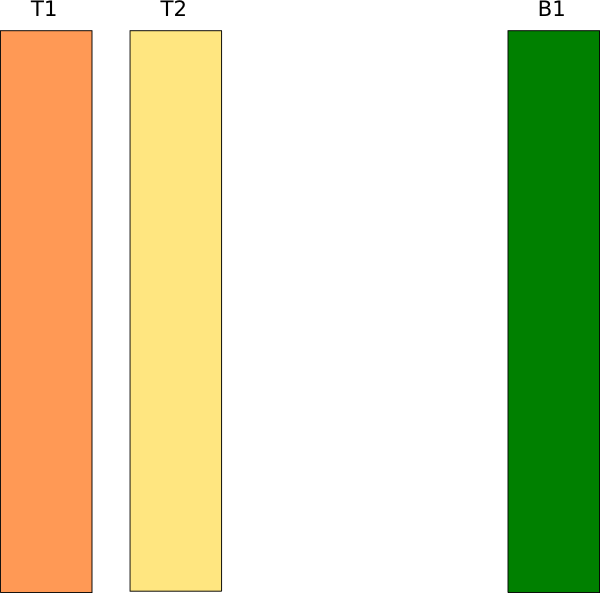
\includegraphics[scale=0.6]{images/shared_buffer_80.png}

\caption{PostgreSQL 8.0, CDB lists}

\end{figure}

The list T1 is used as LRU for the pages loaded from disk. The list T2 is used as LRU list for pages already cached 
and evicted from the list T1. The list B1 is a list of pages recently evicted from the shared buffer.

When a new page is read from disk is put initialy at the beginning of T1. All the CDB in T1 are shifted and the 
last element in T1 is evicted from the shared buffer and his CDB is put at the B1's top.\newline 

\begin{figure}[H]
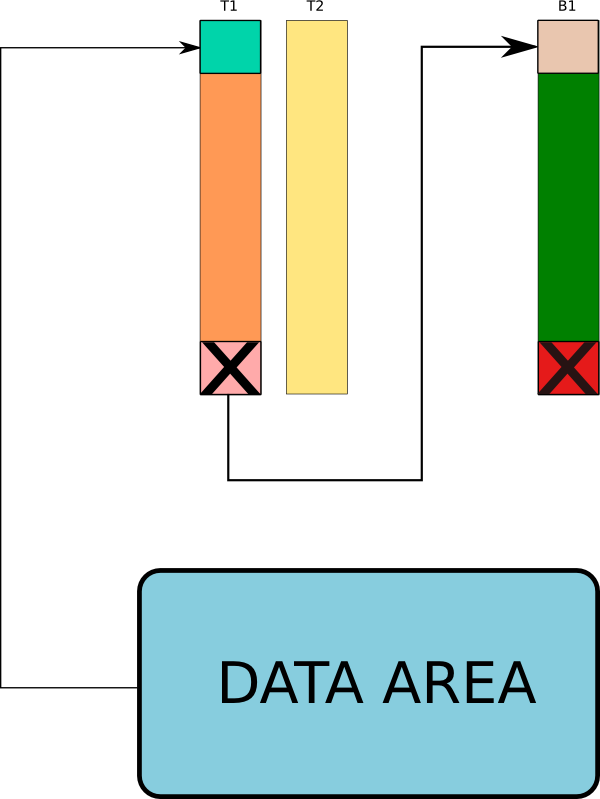
\includegraphics[scale=0.4]{images/2q_01.png}

\caption{2q, read from disk}

\end{figure}

When a backend requests a page present in T1 its CDB is removed from T1 and placed at the T2's top. The last 
element in T2 is  evicted from the shared buffer and its CDB is put at the B1's top.\newline

\begin{figure}[H]
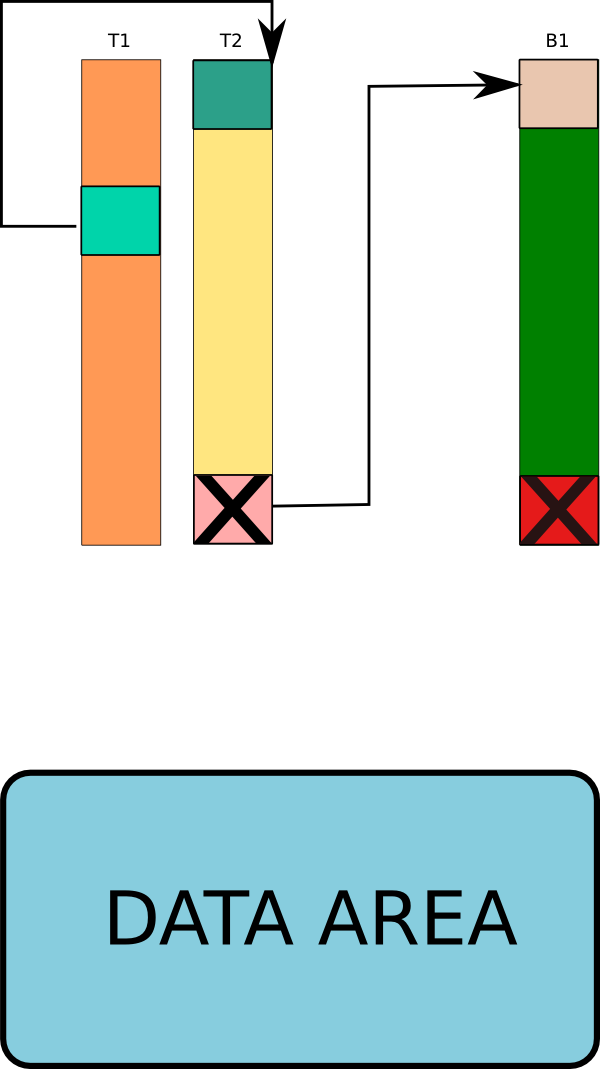
\includegraphics[scale=0.4]{images/2q_02.png}

\caption{2q, page in T1}

\end{figure}

When a backend requests a page in T2 the CDB is moved to the list's top.\newline

\begin{figure}[H]
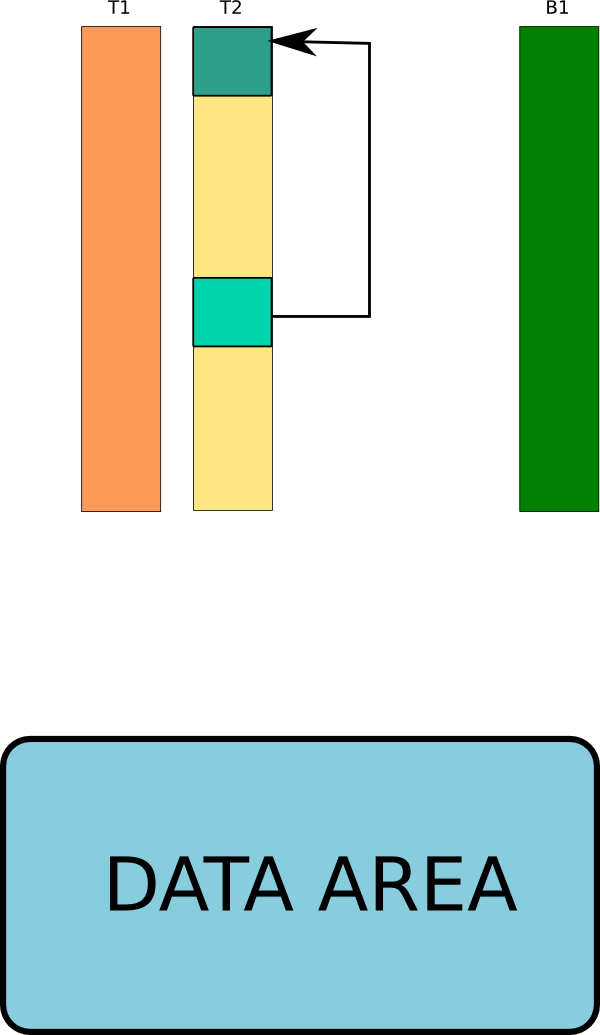
\includegraphics[scale=0.4]{images/2q_03.png}

\caption{2q, page in T2}

\end{figure}

Finally, when a page is read from disk and its CDB is present in B1 then the page is put into T2 instead of 
T1.\newline

\begin{figure}[H]
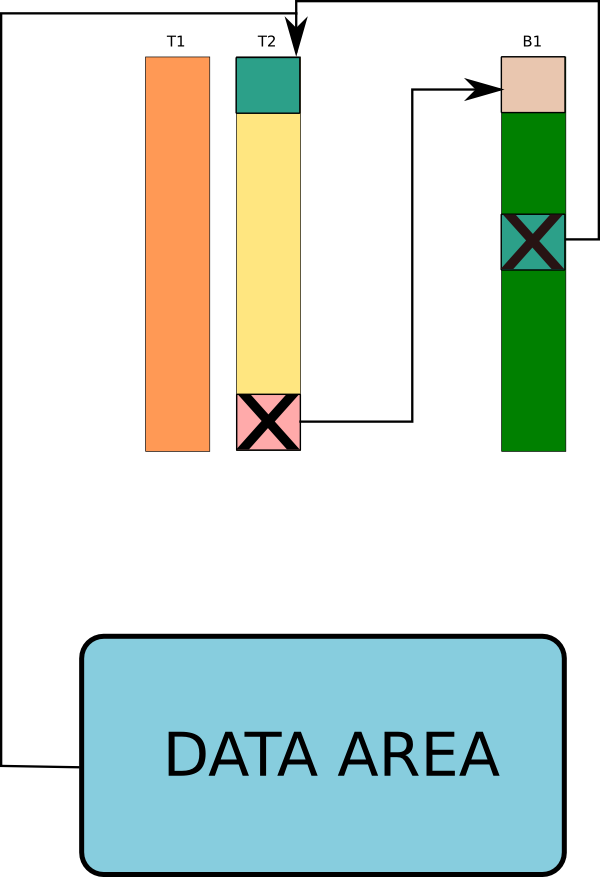
\includegraphics[scale=0.4]{images/2q_04.png}

\caption{2q, page in B1}

\end{figure}

The list T1 acts like a LRU list where the pages requested only one time are evicted quickly if no longer required. 
The list T2 acts like a MRU list where the pages are moved back on the top when required and where the pages from 
T1 are stored if required more than once. The list B1 is used as extra cache to track pages recently evicted from 
the shared buffer that need to stay in T2 if requested again.\newline

Because PostgreSQL can access the page buffers twice when pinning the buffer, in order to avoid the page stored in 
T1 to be moved immediately in T2, the 2q was modified in the evaluation process. The tricky process has shown no 
brilliant performances in production.


\subsubsection{the ARC}
The 2q algorithm was an emergency implementation caused by a software patent held on the algorithm initially 
chosen for the PostgreSQL 8.0's memory manager. Old books, printed meanwhile the 8.0 was in development 
wrongly list the ARC as memory manager. The ARC is an efficient algorithm which keeps in memory two 
lists of page buffers, one for the LRU and for the MRU. Each list adapts dynamically with the different requests 
of the cluster's activity. 

\subsection{PostgreSQL 8.1, the clock sweep}

\subsection{PostgreSQL 8.2, the ringh buffers}

\subsection{PostgreSQL 9.3, SHMMAX no more}
%todo, the change of memory allocation method happened with the 9.3

\subsection{PostgreSQL 9.4, huge pages}

\subsection{The tale of the buffer}
I've read this interesting description years ago on the Bruce Momjian website and explains very well how a 
minimal change can dramatically degrade the database performance.\newline

Our tale will start with a PostgreSQL 7.4 with a 1000 buffers allocated into the shared memory. The page 
size is the default, 8192 bytes. We have in total \begin{math}8192 * 1000 = 8192000\end{math} bytes. On the 
data area we have a full packed table without indices which is consuming 1000 pages on the disk. If we run 
a simple select from the table PostgreSQL  will execute the table's sequential scan in order to get the 
buffers in memory. The sequential is a top to bottom operation. But the shared buffer stores the buffers in 
reverse order. After the initial read, that will take some time because the disk IO, the table fits 
completely into the shared buffer with the pages in reverse order. A second select will find start another 
sequential scan. The buffer manager will search for the table's pages into the shared buffer and will find 
the first table's page into the last slot of the LRU list. This will cause the page move from the last slot 
to the first. The other buffers will shift by one slot all togheter and the second table's page will move 
into the last LRU slot. The buffer manager will find the second table's page in memory and will move the 
page into the first LRU slot causing the buffers shift again. The final result is a faster read because the 
table is totally read from the memory.\newline

Let's add a new row to our table. Because is fully packed this will cause a new page to be added to the 
table which page's count becomes 1001. A select with the shared buffer empty will take the same time of the 
previous condition with one notable exception. When the page 1001 is read from disk the first table's page 
is evicted from the shared buffer to make room. The second select will search for the first table's page 
and it will read from the disk, evicting the second page from the shared buffer. Which is read from disk a 
moment later causing the third page eviction and so on. One single extra page causes the cache spoil. This 
is a corner case of course but tells us an important lesson on the database nature. They are discreet 
systems and most of their behaviour is triggered. Usually there is no soft transition between good and bad
performance. 

\subsection{The wal buffers}

\subsection{The memory manager}
\section{The user memory}
\subsection{Work memory}
\subsection{Maintenance work memory}
\subsection{Temporary memory}


\subsection{Memory context}

\section{Wrap up}